\section{Muhammad Reza Syachrani (1174084)}
\subsection{Teori}

\subsubsection{Apa Itu Random Forest}

\hfill\break
Random Forest merupakan sebuah algoritma yang digunakan pada klasifikasi data dalam jumlah yang besar. Klasifikasi pada random forest dilakukan dengan penggabungan dicision tree dengan melakuakn training terhadap sempel data yang dimiliki. Dengan menggunakan dicision tree yang banyak akan mempengaruhi akurasi yang akan didapatkan menjadi lebih baik. Penentuan klasifikasi dengan random forest sesuai dengan hasil voting dari tree yang terbentuk.
\begin{figure}[H]
\centerline{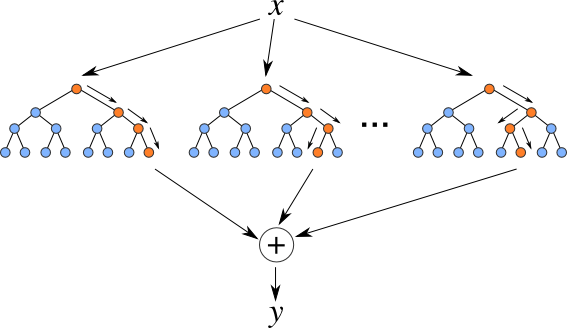
\includegraphics[width=10cm]{figures/1174084/3/1.png}}
\caption{Random Forest}
\label{labelgambar}
\end{figure}

\subsubsection{cara membaca dataset kasus dan artikan makna setiap file dan isi field masing-masing file.}

\hfill\break
Dataset adalah kumpulan data. Paling umum satu data set sesuai dengan isi tabel database tunggal, atau matriks data statistik tunggal, dimana setiap kolom tabel mewakili variabel tertentu,dan setiap baris sesuai dengan anggota tertentu dari dataset yang dipertanyakan. cara membaca dataset :
\begin{itemize}
\item Pertama download dataset terlebih dahulu lalu buka dengan menggunakan software spyder guna melihat isi dari dataset tersebut.

\item Data tersebut memiliki extensi file bernama .txt dan didalamnya terdapat class dari field.

\item Misalnya saja pada data jenis burung memiliki file index dan angka, dimana index berisi angka yang memiliki makna berupa jenis burung.

\item bahkan nama burung sedangkan field memiliki isi nilai berupa 0 dan 1 yang dimana sifatnya boolean atau Ya dan Tidak.

\item Hal ini dikarenakan komputer hanya dapat membaca bilangan biner maka dari itu field yang di isikan berupa angka.

\item Artinya angka 0 berarti tidak dan angka 1 berarti Ya.
\end{itemize}

\subsubsection{Cross Validation}

\hfill\break
Cross Validation adalah teknik validasi model untuk menilai suatu hasil statistik analisis yang akan menggeneralisasi kumpulan data independen. Teknik ini digunakan untuk melakukan prediksi model dan memperkirakan seberapa akurat sebuah model prediktif ketika dijalankan dalam praktiknya. Tujuan dari cross validation adalah untuk mendefinisikan dataset untuk menguji model dalam tahap pelatihan (yaitu, validasi data), dalam rangka untuk membatasi masalah seperti terjadinya overfitting, memberikan wawasan tentang bagaimana model dapat menggeneralisasi independen dataset.
\subsubsection{Arti score 44 \% pada random forest, 27\% pada decission tree dan 29 \% dari SVM.}

\hfill\break
Dimana Score 44 \% didapatkan dari hasil pengelohan dataset jenis burung. Dimana akan dilakukan proses pembagian data testing dan data training lalu diproses dan menghasilkan score sebanyak 44 \% dimana menjelaskan bahwa score tersebut digunakan sebagai pembanding dalam tingkat keakuratannya. Pada dicision tree akan memperoleh data lebih kecil yaitu sebanyak 27 \% hal ini dikarenakan data yang diolah menggunakan dicision tree dibagi menjadi beberapa tree dan lalu disimpulkan untuk mendapatkan data yang akurat. Pada SVM akan memperoleh score sebanyak 29 \% hal ini dikarenakan data yang dimiliki masih bernilai netral sehingga tingkat keakuratannya masih belum jelas.

\subsubsection{Cara membaca confusion matriks dan contohnya memakai gambar atau ilustrasi sendiri.}

\hfill\break
Perthitungan Confusion Matriks dapat dilakukan dengan cara dibawah ini.
\begin{itemize}
\item
Import librari Pandas, Matplotlib, dan Numpy.
\item
Buat variabel y actu yang isinya berupa data aktual.
\item
Buat variabel y pred berisikan data yang akan dijadikan sebagai prediksi.
\item
Buat variabel df confusion yang berisikan crosstab untuk membangun tabel tabulasi silang yang dapat menunjukkan frekuensi kemunculan kelompok data tertentu.
\item
Pada variabel df confusion definisikan lagi nama baris yaitu Actual dan kolomnya Predicted
\item
Kemudian definisikan suatu fungsi yang diberi nama plot confusion matrix yang berisikan pendefinisian confusion matrix dan juga akan di plotting.
\lstinputlisting{src/1174084/3/confusion.py}
\end{itemize}
\begin{figure}[H]
\centerline{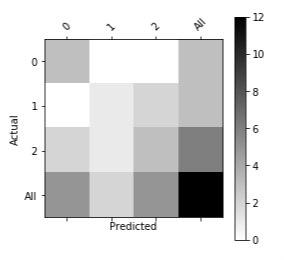
\includegraphics[width=10cm]{figures/1174084/3/2.png}}
\caption{Confusion Matriks}
\label{labelgambar}
\end{figure}

\subsubsection{Apa itu voting pada random forest}

\hfill\break
Voting yaitu suara untuk setiap target yang diprediksi pada saat melakukan Random Forest dilakukan. Pertimbangkan target prediksi dengan voting tertinggi sebagai prediksi akhir dari algoritma random forest.

\begin{figure}[H]
\centerline{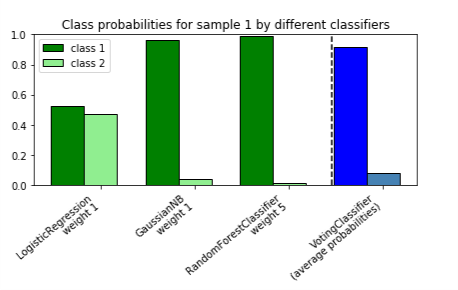
\includegraphics[width=10cm]{figures/1174084/3/3.png}}
\caption{Voting Random Matriks}
\label{labelgambar}
\end{figure}


\subsection{Praktek}
\subsubsection{Nomor 1}
\hfill\break
\lstinputlisting[firstline=9, lastline=15]{src/1174084/3/1174084.py}
\begin{figure}[H]
\centerline{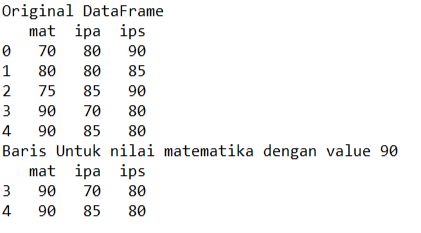
\includegraphics[width=10cm]{figures/1174084/3/4.png}}
\caption{Membuat Aplikasi pakai pandas}
\label{labelgambar}
\end{figure}

\subsubsection{Nomor 2}
\hfill\break
\lstinputlisting[firstline=19, lastline=29]{src/1174084/3/1174084.py}
\begin{figure}[H]
\centerline{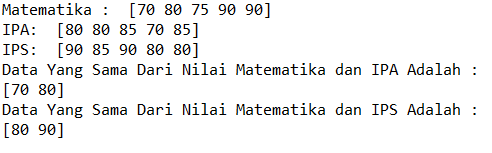
\includegraphics[width=10cm]{figures/1174084/3/5.png}}
\caption{Membuat Aplikasi pakai numpy}
\label{labelgambar}
\end{figure}

\subsubsection{Nomor 3}
\hfill\break
\lstinputlisting[firstline=33, lastline=56]{src/1174084/3/1174084.py}
\begin{figure}[H]
\centerline{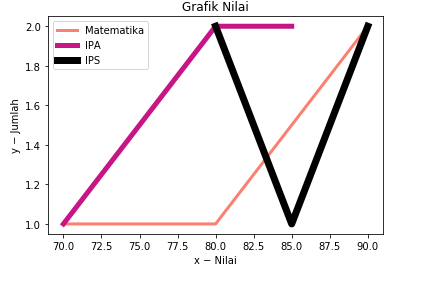
\includegraphics[width=10cm]{figures/1174084/3/6.png}}
\caption{Membuat Aplikasi pakai matplotlib}
\label{labelgambar}
\end{figure}

\subsubsection{Nomor 4}
\hfill\break
\lstinputlisting[firstline=60, lastline=108]{src/1174084/3/1174084.py}
\begin{figure}[H]
\centerline{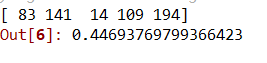
\includegraphics[width=10cm]{figures/1174084/3/7.png}}
\caption{Hasil Random Forest}
\label{labelgambar}
\end{figure}

\subsubsection{Nomor 5}
\hfill\break
\lstinputlisting[firstline=112, lastline=115]{src/1174084/3/1174084.py}
\begin{figure}[H]
\centerline{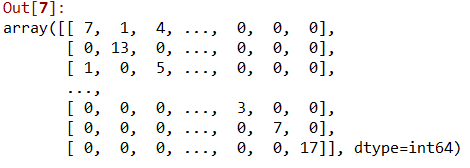
\includegraphics[width=10cm]{figures/1174084/3/8.png}}
\caption{Hasil Confusion Matrix}
\label{labelgambar}
\end{figure}

\subsubsection{Nomor 6}
\hfill\break
\lstinputlisting[firstline=11, lastline=120]{src/1174084/3/1174084.py}
\begin{figure}[H]
\centerline{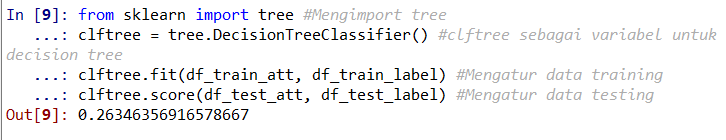
\includegraphics[width=10cm]{figures/1174084/3/9.png}}
\caption{Hasil Decision Tree}
\label{labelgambar}
\end{figure}

\subsubsection{Nomor 7}
\hfill\break
\lstinputlisting[firstline=123, lastline=125]{src/1174084/3/1174084.py}
\begin{figure}[H]
\centerline{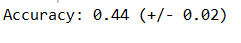
\includegraphics[width=10cm]{figures/1174084/3/10.png}}
\caption{Hasil Cross Validation}
\label{labelgambar}
\end{figure}

\subsubsection{Nomor 8}
\hfill\break
\lstinputlisting[firstline=129, lastline=143]{src/1174084/3/1174084.py}
\begin{figure}[H]
\centerline{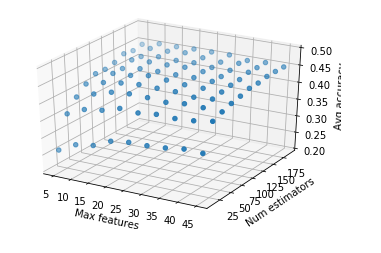
\includegraphics[width=10cm]{figures/1174084/3/11.png}}
\caption{Hasil Pengamatan }
\label{labelgambar}
\end{figure}

\subsection{Penanganan Error}
\begin{enumerate}
	\item ScreenShoot Error
	\begin{figure}[H]
		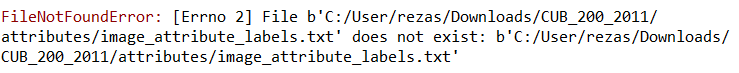
\includegraphics[width=4cm]{figures/1174084/3/error1.png}
		\centering
		\caption{FileNotFoundError}
	\end{figure}
	\item Tuliskan Kode Error dan Jenis Error
	\begin{itemize}
		\item FileNotFoundError
	\end{itemize}
	\item Cara Penangan Error
	\begin{itemize}
		\item FileNotFoundError
		\hfill\break
		Error terdapat pada kesalahan saat baca file csv, yang tidak terbaca. Dikarenakan letak file yang dibaca tidak pada direktori yang sama. Seharusnya letakkan file di direktori yang sama. 
	\end{itemize}
\end{enumerate}


\subsection{Bukti Tidak Plagiat}
\hfill\\
\begin{figure}[H]
\centerline{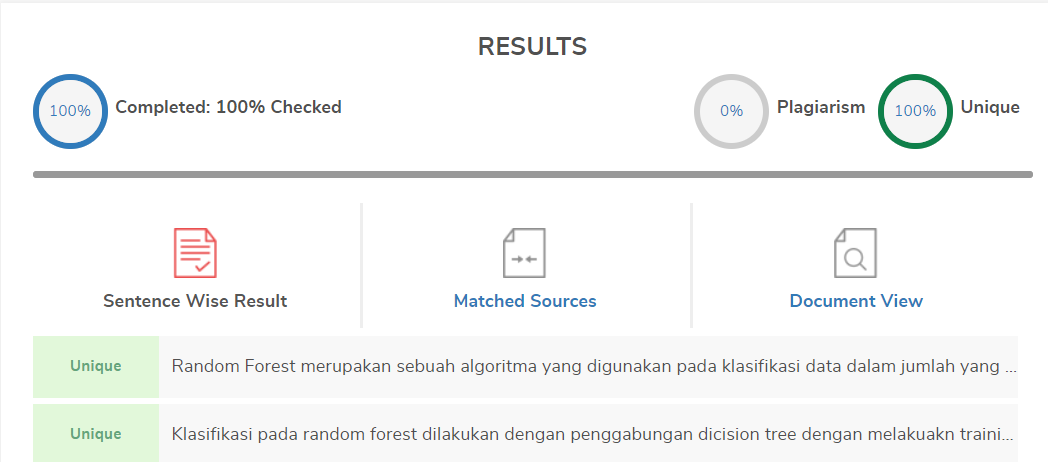
\includegraphics[width=10cm]{figures/1174084/3/plagiat.png}}
\caption{Bukti Tidak Plagiat}
\label{labelgambar}
\end{figure}

\subsection{Link Youtube:}
https://youtu.be/qtmtKsziZ1I